\documentclass[11pt, english]{article}

\usepackage{multicol}
\usepackage{hyperref}
\usepackage[eng]{felipito}
\usepackage{stfloats}
\usepackage{mathpazo}

\usepackage[margin=0.7in, left=0.7in, right=0.7in]{geometry}

\graphicspath{{./Graphics/}}

% Colors
\definecolor{urlcolor}{rgb}{0,.145,.698}
\definecolor{linkcolor}{rgb}{.71,0.21,0.01}
\definecolor{citecolor}{rgb}{.12,.54,.11}


% Document title
\title{\bf Problem Set 5 \\ Statistics, Computation and
Applications\\[-1ex]}
\author{Felipe del Canto}
\date{November, 2021}
    
\hypersetup{
	breaklinks=true,  % so long urls are correctly broken across lines
    colorlinks=true,
    urlcolor=urlcolor,
    linkcolor=linkcolor,
    citecolor=citecolor,
}

\begin{document}
    
\maketitle
   
\begin{multicols}{2}

\section*{Problem 5.1: Flows and Correlations}

For parts (a) and (b), the first step is to compute the average flow over time. The grid used implies that each coordinate covers a 3km grid. Additionally, all flow values are expressed in cm/second (cmps). In order to gain a better sense of the strength of the currents, two different average speeds are computed. First, the speed of the average flow. This is, compute the speed \textit{after} averaging the flow vectors. Second, the average of all speed values over time. In other words, the speed is \textit{before} averaging. In \Cref{fig:flow-speed} it is presented the first of these two speed representations. The fastest flow runs from east to west on the southern end of the Archipielago (around 900 km east of the initial coordinate). There is also a strong current around the islands to the southwest (around 300 km north of the initial coordinate) Other important flows run on the east, mostly going south. There are lesser important but prevalent currents running almost in circular patterns at the center and the west and at the center-north, on the east. In contrast, in \Cref{fig:flow-speed-2} is presented the second of the speed representations. In this case, the speed of the flow at each time is computed and then averaged over time. The patters shown in the previous picture still hold. The most strong currents are present in the southern part of the Archipielago, and in the islands at the south west (around 900 km to the north of the initial coordinates).

For part (c), the main goal is to understand if a Gaussian Process (GP) might be a good model for making predictions about currents in the Archipielago. For this, spatial correlations must be understood. To this end, two coordinates are considered and the flow and speed correlations with their surroundings are studied. The two coordinates are (420 km, 345 km) and (1200 km, 1200 km). Moreover, the correlations are computed for three variables: the horizontal flow, the vertical flow and the speed. In \Cref{fig:coord} are presented the results for both coordinates. In particular, panels (a) to (c) show the correlations for the first coordinate. These figures show that horizontal flow is more diverse in terms of correlation, with zones close to the point of reference that have high and low correlation values. On the opposite side, the vertical component of the flow is in general more positively correlated with the reference point. In particular, the previous observation suggests that a GP would not be a reasonable model for the horizontal component of the flow. This, because the red zones are roughly at the same distance that other blue zones. If a GP with covariances following a kernel modelled these zones, then both should have the same color. Additionally, the zones south of the reference point do not seem correlated with it, mounting more evidence against a GP model. In contrast, the vertical component and speed images do have a more stable behavior in terms of the neighbors of the reference point. However, the same concern regarding zones more to the south suggests that GP is not a good model. Now, we turn to the surroundings of the second coordinate, which are shown in \Cref{fig:coord-2-h,fig:coord-2-v,fig:coord-2-s}. These panels show a completely different story. Around the reference point, the correlations are spurious. In particular, the zones closer to the point have almost zero correlation. In that sense, it could be argued that in this case, GP are a good model. However, the small correlations would imply a very poor predictive power, making the model useless nonetheless. In the other hand, the caveat is that even if the surroundings of the reference point do follow a distance-driven covariance pattern, points further away have nonzero correlations. If a GP were to model this data, the correlation between the reference point and these far away points should be smaller than those closer, which is not the case. All in all, the analysis of the previous two coordinates suggests that a GP would not be a good model for this data. The reason might be that currents form a complex system, with difficult rules. If these rules are nonlinear, then correlations, that are more suited for linear dependencies, fail to capture the underlying phenomena.

\section*{Problem 5.2: Predicting Trajectories}

For part (a), the goal is to implement a procedure to track the position and movement of a particle moving through the ocean flow given by the data. The following approach is considered. Given initial coordinates $(x_0, y_0)$, the movement of the particle is simulated in a second-to-second basis. This is, the new position of the particle is computed every second. The flow that governs the particle's movement is given by the flow of the grid the particle is in, and the current timestamp $T \in \{1, \ldots, 100\}$. Note that computing the movement in this fashion induces a minor estimation error. However, this is negligible given the size of the grid (3 km) and the timeframe considered (300 hours). In \Cref{fig:test-simulations} are presented four simulations with different starting points. The red dot presents the initial point, while the blue lines represent the trajectory.

For part (b), a toy plane crashed at $T=0$ in the Sulu Sea. The exact location of the crash is unknown, but estimates suggest the location follows a Gaussian distribution with mean (100 km, 350 km) and variance $\sigma^2 I$. The goal is to estimate where the plane debris will be after 48, 72 and 120 hours. The results will be compared when the variance is 25 km, 50 km, and 100 km. In \Cref{fig:toy} are presented the results of simulating samples from each distribution and determining the potential position of the debris for 48, 72 and 120 hours after the crash. In general, the current around the crash site is not intense (see \Cref{fig:flow}) and even after 120 hours, the debris have not moved far. Nevertheless, interesting patterns appear between the images. As expected, the longer the time of the journey, the farthest the debris travel. This implies that the blue lines are longer on the images on the right than the ones on the left. However, the most interesting phenomena is that as the variance increases, the actual location could have been in a more turbulent area of the sea, making the debris move longer distances in a short amount of time. For example, comparing \Cref{fig:toy-48-25} and \Cref{fig:toy-48-50} it is possible to observe that some of the potential trajectories are longer, since the simulated crash occurred in an area where the flow was stronger. 


\section*{Problem 5.3: Gaussian Processes}

For part (a), consider the squared exponential/RBF covariance function
	$$\kappa(x_{i}, x_{j}) = \sigma^{2}\exp\left(-\frac{(x_{i} - x_{j})^{2}}{2\ell^{2}}\right),$$
where $\sigma^2$ is the signal variance and $\ell$ is the lengthscale. If the signal variance is increased, then all things equal, points will have a higher covariance. In other words, the covariance curve (as a function of distance $|x_{i} - x_{j}|$) is higher, the higher $\sigma^{2}$ is. This is shown in \Cref{fig:rbf-sigma}. Moreover, the image shows the decay is similar among all three functions, reaching values close to zero when the distance is close to 3. On the other hand, varying the lengthscale has different effects on the covariance function. As shown in \Cref{fig:rbf-ell}, changing the lengthscale drastically affects the decaying rate of the function. When $\ell$ is small, the decay is faster than when it is larger.

For parts (b) and (c), suppose we have data points $\{(x_{i}, y_{i})\}_{i=1}^{N}$, where $x_{i}$ are locations and $y_{i}$ are given outcomes. Additionally, we have a new observation $x_{*}$ for which we wish to estimate $y_{*}$. A Gaussian Process (GP) model assumes each $y_{i}$ is drawn from $Y_{i}$ and that $Y := (Y_{1}, \ldots, Y_{N}, Y_{*})$ follows a multivariate normal distribution. Let $\mu$ and $\Sigma$ be the mean and covariance matrix of that distribution and assume $\mu = 0$. Let $\sigma_{*}$ be the variance of $Y_{*}$, $\sigma_{N}$ be the $N \times N$ top left block of $\Sigma$, and let $k^{*}$ be the vector whose entries are $k(x_{*}, x_{i})$, where $k$ is the kernel function that is used to model the covariances. Then, the parameters for the distribution of $Y_{*}$ are:
	\begin{align*}
		\mu_{*\,|\,1:N}		&=	k_{*}^{T}K_{N}^{-1}y_{1:N}	\\
		\sigma_{*\,|\,1:N}	&=	\sigma_{*} - k_{*}^{T}K_{N}^{-1}k_{*}
	\end{align*}
Observe that computing both parameters implies that the matrix $K_{N}$ has to be inverted. If $N$ is large, this operation can take large amounts of time or even be impossible to do due to memory restrictions. In order to do this computation more efficient, an option is to compute the singular value decomposition (SVD) of $K_{N}$. However, the problem persists unless we are willing to approximate the SVD. For this, we can take the algorithm proposed by Halko et al.\footnote{Halko, N., Martinsson, P.-G., \& Tropp, J. A. (2011). Finding structure with randomness: Probabilistic algorithms for constructing approximate matrix decompositions. SIAM Review, 53(2), 217–288.} In their  framework, given $K_{N}$, the idea is to find an orthonormal $N \times \ell$ matrix $Q$ with $\ell \leq N$ columns such that $QQ^{T}K_{N} \approx K_{N}$. Then, setting $B := Q^{T}K_{N}$, compute the SVD of $B$, $B = \overline{U}\Sigma V^{T}$ and produce a low-rank approximation of $K_{N}$ by setting $U = Q^{T}\overline{U}$ and obtaining $K_{N} = U\Sigma V^{T}$. To find $Q$, the algorithm tries to obtain it by setting a tolerance $\epsilon$ and finding $Q$ such that
	$$\|A - QQ^{*}A\| \leq \epsilon$$
This can be done by building $Q$ incrementally in similar fashion as the Gram-Schmidt process. This last step involves drawing random gaussian vectors that help mapping the range of $K_{N}$. Since the SVD is computed in a smaller matrix than $K_{N}$ the process is faster. The hyperparameter $\ell$ determines both the quality of the final approximation and how much the process is speeded.

\begin{figure*}
	\caption{Average flow and speed flow for a zone of the Philippines Archipielago. In panel (a), the rows represent the average flow over time. The colors on the arrows represent the speed of the flow (i.e., the size of the arrow) in cmps. In panel (b), the colors represent the average speed over time, that is, averaging the speed of the flow at each time.}
	\label{fig:flow}
	\begin{subfigure}{0.48\textwidth}
		\centering
		\caption{Average flow and speed}
		\label{fig:flow-speed}
		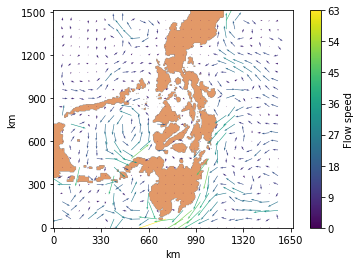
\includegraphics[width=\textwidth]{flow-speed}
	\end{subfigure}\hfill
	\begin{subfigure}{0.48\textwidth}
		\centering
		\caption{Average speed over time}
		\label{fig:flow-speed-2}
		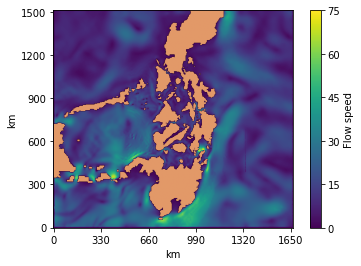
\includegraphics[width=\textwidth]{flow-speed-2}
	\end{subfigure}
\end{figure*}

\begin{figure*}
	\caption{Spatial correlations for coordinates (420 km, 345 km) and (1200 km, 1200 km). Panels (a)-(c) show the correlations of the first coordinate and its surroundings for horizontal flow, vertical flow, and speed, respectively. Analogously, panels (d)-(f) show the same for the second coordinate. In all panels, the green dot represents the corresponding coordinate.}
	\label{fig:coord}
	\begin{subfigure}{0.33\textwidth}
		\centering
		\caption{Horizontal flow.}
		\label{fig:coord-1-h}
		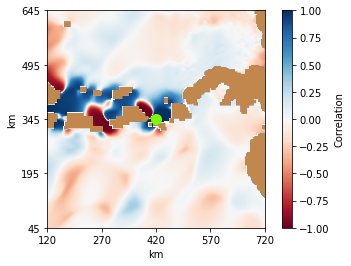
\includegraphics[width=\textwidth]{coord-1-h}
	\end{subfigure}\hfill
	\begin{subfigure}{0.33\textwidth}
		\centering
		\caption{Vertical flow.}
		\label{fig:coord-1-v}
		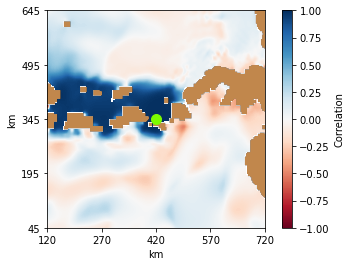
\includegraphics[width=\textwidth]{coord-1-v}
	\end{subfigure}
	\begin{subfigure}{0.33\textwidth}
		\centering
		\caption{Speed.}
		\label{fig:coord-1-s}
		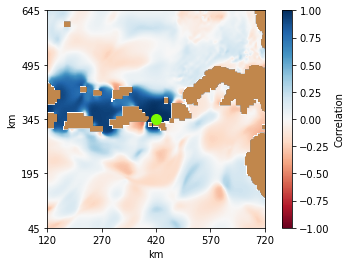
\includegraphics[width=\textwidth]{coord-1-s}
	\end{subfigure}\vspace{2ex}
	
	\begin{subfigure}{0.33\textwidth}
		\centering
		\caption{Horizontal flow.}
		\label{fig:coord-2-h}
		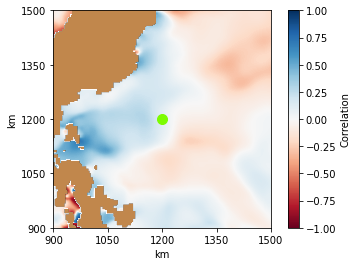
\includegraphics[width=\textwidth]{coord-2-h}
	\end{subfigure}\hfill
	\begin{subfigure}{0.33\textwidth}
		\centering
		\caption{Vertical flow.}
		\label{fig:coord-2-v}
		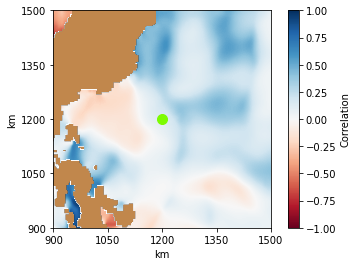
\includegraphics[width=\textwidth]{coord-2-v}
	\end{subfigure}
	\begin{subfigure}{0.33\textwidth}
		\centering
		\caption{Speed.}
		\label{fig:coord-2-s}
		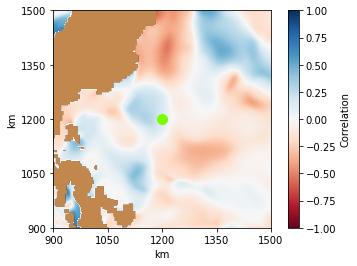
\includegraphics[width=\textwidth]{coord-2-s}
	\end{subfigure}
\end{figure*}

\begin{figure*}
	\caption{Simulation of trajectories of a particle subject to the ocean flow, from a given initial coordinate. The red dot represents the starting point and the blue line represents the journey of the particle.}
	\label{fig:test-simulations}
	\begin{subfigure}{0.48\textwidth}
		\centering
		\caption{(300, 462)}
		\label{fig:test-simulations-1}
		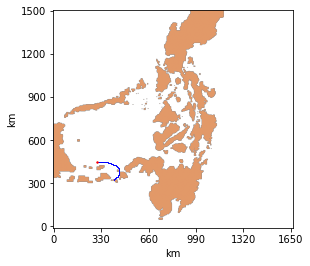
\includegraphics[width=0.75\textwidth]{test-simulations-1}
	\end{subfigure}\hfill
	\begin{subfigure}{0.48\textwidth}
		\centering
		\caption{(600, 1362)}
		\label{fig:test-simulations-2}
		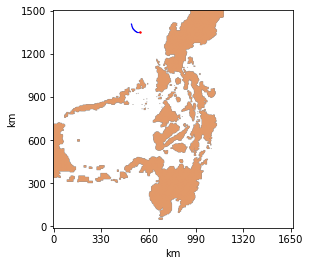
\includegraphics[width=0.75\textwidth]{test-simulations-2}
	\end{subfigure}\vspace{2ex}

	\begin{subfigure}{0.48\textwidth}
		\centering
		\caption{(1320, 252)}
		\label{fig:test-simulations-3}
		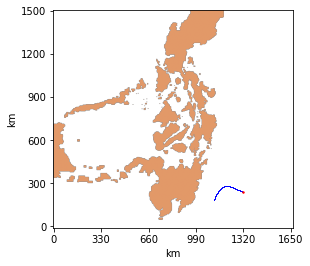
\includegraphics[width=0.75\textwidth]{test-simulations-3}
	\end{subfigure}\hfill
	\begin{subfigure}{0.48\textwidth}
		\centering
		\caption{(1320, 1212)}
		\label{fig:test-simulations-4}
		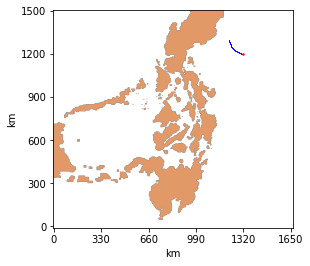
\includegraphics[width=0.75\textwidth]{test-simulations-4}
	\end{subfigure}
\end{figure*}

\begin{figure*}
	\caption{Toy plane possible debris location after 48, 72 and 120 hours for different variances. The red dot and circle represent the distribution up to two standard deviations. The blue lines are potential debris trajectories.}
	\label{fig:toy}
	\begin{subfigure}{0.33\textwidth}
		\centering
		\caption{48 hours, $\sigma^{2} = 25$.}
		\label{fig:toy-48-25}
		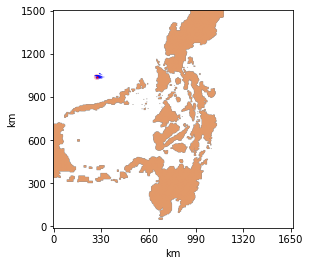
\includegraphics[width=\textwidth]{toy-48-25}
	\end{subfigure}\hfill
	\begin{subfigure}{0.33\textwidth}
		\centering
		\caption{72 hours, $\sigma^{2} = 25$.}
		\label{fig:toy-72-25}
		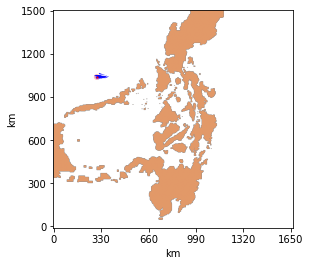
\includegraphics[width=\textwidth]{toy-72-25}
	\end{subfigure}
	\begin{subfigure}{0.33\textwidth}
		\centering
		\caption{120 hours, $\sigma^{2} = 25$.}
		\label{fig:toy-120-25}
		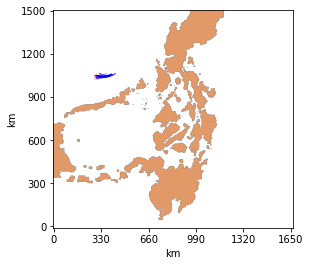
\includegraphics[width=\textwidth]{toy-120-25}
	\end{subfigure}\vspace{2ex}
	
	\begin{subfigure}{0.33\textwidth}
		\centering
		\caption{48 hours, $\sigma^{2} = 50$.}
		\label{fig:toy-48-50}
		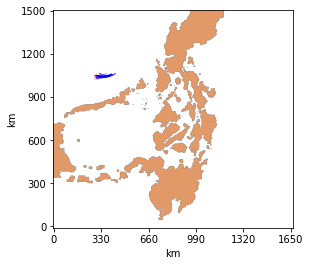
\includegraphics[width=\textwidth]{toy-48-50}
	\end{subfigure}\hfill
	\begin{subfigure}{0.33\textwidth}
		\centering
		\caption{72 hours, $\sigma^{2} = 50$.}
		\label{fig:toy-72-50}
		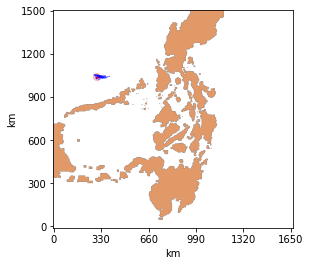
\includegraphics[width=\textwidth]{toy-72-50}
	\end{subfigure}
	\begin{subfigure}{0.33\textwidth}
		\centering
		\caption{120 hours, $\sigma^{2} = 50$.}
		\label{fig:toy-120-50}
		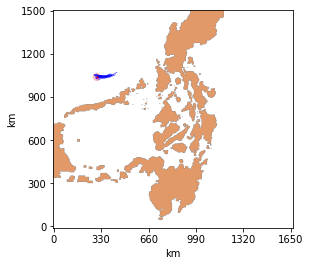
\includegraphics[width=\textwidth]{toy-120-50}
	\end{subfigure}\vspace{2ex}
	
	\begin{subfigure}{0.33\textwidth}
		\centering
		\caption{48 hours, $\sigma^{2} = 100$.}
		\label{fig:toy-48-100}
		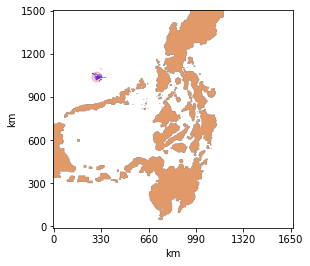
\includegraphics[width=\textwidth]{toy-48-100}
	\end{subfigure}\hfill
	\begin{subfigure}{0.33\textwidth}
		\centering
		\caption{72 hours, $\sigma^{2} = 100$.}
		\label{fig:toy-72-100}
		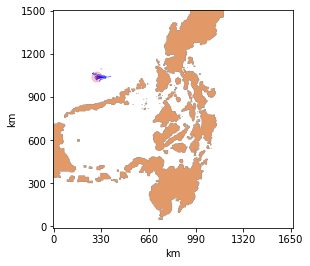
\includegraphics[width=\textwidth]{toy-72-100}
	\end{subfigure}
	\begin{subfigure}{0.33\textwidth}
		\centering
		\caption{120 hours, $\sigma^{2} = 25$.}
		\label{fig:toy-120-100}
		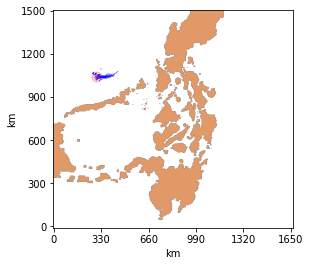
\includegraphics[width=\textwidth]{toy-120-100}
	\end{subfigure}
\end{figure*}

\begin{figure*}
	\caption{Effect of $\sigma^{2}$ and $\ell$ on the RBF covariance function $\kappa(x_{i}, x_{j})$. Panel (a) shows the effect of varying $\sigma^{2}$, when holding $\ell = 1$ constant. In panel (b) it is shown the effect of varying $\ell$, holding $\sigma^{2} = 1$ constant.}
	\label{fig:rbf}
	\begin{subfigure}{0.48\textwidth}
		\centering
		\caption{$\ell = 1$}
		\label{fig:rbf-sigma}
		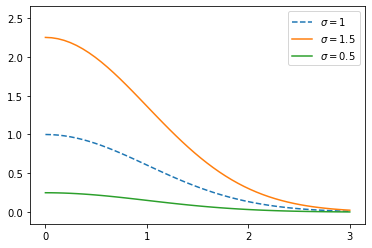
\includegraphics[width=\textwidth]{rbf-sigma}
	\end{subfigure}\hfill
	\begin{subfigure}{0.48\textwidth}
		\centering
		\caption{$\sigma^{2} = 1$}
		\label{fig:rbf-ell}
		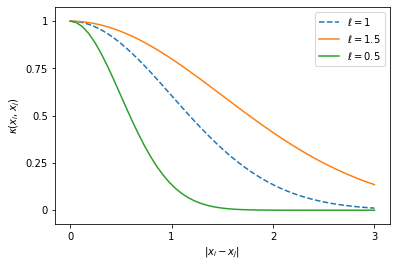
\includegraphics[width=\textwidth]{rbf-ell}
	\end{subfigure}
\end{figure*}


\end{multicols}



\end{document}
